%************************************************
\chapter{Background}\label{ch:background}
%************************************************
This chapter introduces the general concepts on which we build on in this thesis.
We explain the concepts behind \emph{configurable software systems} and afterwards, how we model these configurable software systems with
feature models.           %MAYBE ADD TGE INFLUECNE ON THE PERFORMANCE
We introduce \emph{performance-influcence models}, a way to model and predict the influcence of features on the configurable software system.
In \autoref{ch:Blackbox} and \autoref{ch:Whitebox}, we introduce \emph{black-box analysis} and \emph{white-box analysis}, 
two different analysis approaches to analyze the performance of configurable software systems.

\section{Configurable Systems}\label{ch:configurable-systems}
\theoremstyle{definition}
\newtheorem{definition}{Definition}[section]

In this section, we start of explaining the general concepts behind configurable systems and the reason for using them. 
We proceed with explaining what a feature and configuration is in \autoref{feature-config}. 
Additionally, we introduce functional and non-functional properties in \autoref{ch:properties} and show the difference between them.

\subsection{General Concepts}\label{ch:general-concepts}
%What is a Conf. system and why we use it
We call a system configurable if it offers options that allow developers and end-users to turn functionality on and off.
This gives the system the benefit of satisfying the demand of multiple user groups by providing a single software system containing various features
~\cite{TooManyKnobs}.


\begin{figure}[h]
    \centering
    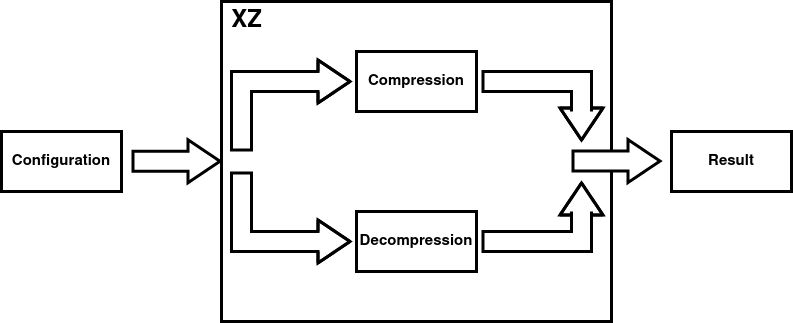
\includegraphics[scale=0.55]{gfx/ConfigurableSystemXZ.png}
    \caption{Simplified version of \textsc{XZ}.}
    \label{fig:xz}
\end{figure}

%Example for such a system using xz
As an example, let us inspect the compression tool \textsc{XZ}\footnote{Visited at 21.03.2023 \url{https://tukaani.org/xz/}}.
In \autoref{fig:xz} depicts a simplified version of \textsc{XZ}, which contains two main functions, encryption, and decryption. 
It is up to the user to decide what he needs, but regardless of his choice, a single software system contains both functions.

\subsection{Features and Configurations}\label{feature-config}

%What is a feature
During the years there have been many definitions to what a \emph{feature} is, on one side, features are used as a means of communication between
the different stakeholder of a system, where on the other hand, a feature is defined as an implementation-level concept. 
To unify both applications Apel et.al. introduced the following definition~\cite{Feature-Oriented-Software-Product-Lines}:

%Definition
\begin{definition}
    "A structure that extends and modifies the structure of a
    given program in order to satisfy a stakeholder's requirement, to implement and
    encapsulate a design decision, and to offer a configuration option."     
\end{definition}

%Example of feature on xz an definition of configuartion
Thus, a feature is both an abstract concept that refers to particular functionality of a system and the implementation of that functionality.
In our example \autoref{fig:xz} both, \textit{Compression} and \textit{Decompression}, are unique features, they refer to a piece of functionality of the system and the
implementation. 

%Numeric and binary feature
We differentiate between \emph{binary} features \emph{numeric} features. A binary feature can be either selected or deselected; 
commonly, we denote a binary feature with $1$ if we select it and $0$ otherwise. 
We denote a numeric feature with a numerical value; these can have various meanings depending on the feature it implements. 
For \autoref{fig:xz}, \textit{Decompression} could be a binary feature since we either have the option to decrypt a file or not; on the contrary, 
\textit{Compression} could be implemented as a numeric feature, where the numeric value represents the quality of compression we want. 

%What is a Configuration option
A configuration option is a predefined way for developers to change the functionality of the configurable system; 
these options allow us to select features we want to include or exclude. Thus, a configuration is a set of configuration options, whereas 
we call a configuration valid as long as it satisfies the system's constraints.

%What is a Configuration space
The configuration space refers to the set of all configurations. However, some of these configurations are invalid. 
In practice, we cannot execute systems with invalid configurations. 
Therefore, we shall implicitly exclude all invalid configurations whenever we refer to a configuration space.

%Example
As an example, \textsc{XZ} offers the user different features such as \textit{Compression} and \textit{Decompression}, whereas 
the configuration options \textit{0-9} specify the degree of compression. An invalid configuration would be to select multiple 
degrees of compression.

\section{Functional and Nonfunctional Properties}\label{ch:properties}

When analyzing a configurable system we can divide the properties of that system into two categories, functional and non-functional properties.
As functional properties 

\section{Modelling Configurable System}\label{ch:modelling-configsys}

In this section, we explain how we model configurable systems using \emph{feature models}. 
Furthermore, we introduce \emph{feature diagrams}, a visual representation of feature models.

\chapter{Feature Model}\label{ch:Feature Model}

\begin{figure}[h]
    \centering
    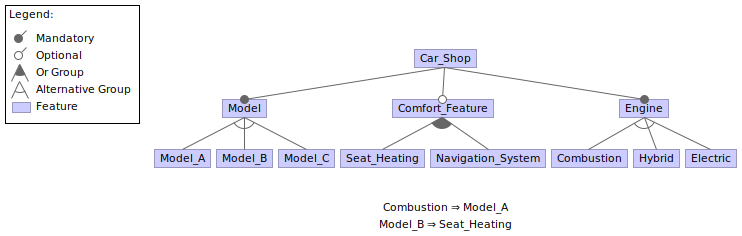
\includegraphics[scale=0.6]{gfx/Car_Shop.png}
    \caption{A feature model of a car shop}
    \label{fig:car}
\end{figure}

A configurable system often contains numerous features, all these features might interact with one another or have different dependencies.
To help us keep a overview of the system we introduce feature model \cite{Feature-Oriented-Software-Product-Lines-Feature-models}. A example
of a feature model for a car shop can be found in \ref{fig:car}

A feature model is essentialy a tree, that models a configurable system, each node in that tree represent a specific feature whereas the root
represent the system itself. If a feature is selected it implies that also the parent of that features needs to be selected as well, the further
we decend in the tree the more specific features get. In \ref{fig:car} we see Engine is a feature where as the children a concrete types
of engines, specificly Combustion, Hybrid and Electric.

Each feature may contain a grafical notation to indicate whether the feature is mandatory or optional, if the feature is mandatory, it is 
indicated with a black bubble and if its optional its optional its indicated with a empty bubble, in \ref{fig:car} we can see that Engine and
Model are mandatory features, which make sense since both are necessary for each car, but Comfort\_Feature a optional since they are not
necessary for a car to function.

Besides mandatory and optional feature we also have alternative and choice groups. A parent can have one of these groups, a alternative group
is denoted with a empty half circle and a optional group with a filled circle. If a choice group is used, one feature needs to be selected, but
others can be selected as well, a choice group corresponds to the logical or operator. In a alternative group, one and only one feature can be
selected, if more the one is selected the configuration is invalid. In \ref{fig:car} we see Engine has a alternative group, which makes sense
since each car can only contain one Engine, where it makes sense that Comfort\_Feature contains a choice group, you can have a navigation system
and seat heating in a car without any conflics.

In addition to that, a feature model can contain different constraints that need to be satisfied, these constraints are defined as boolean 
algebra. In \ref{fig:car} we can see that there are two constraints, $Combustion \implies Model\_A$ and 
$Model\_B \implies Seat\_Heating$, the reasons for such constraints could be that Model\_B is a luxurious model where it only gets shipped
with seat heating.

Every feature model can also be translated into compositional logic \cite*{Feature-Oriented-Software-Product-Lines-Feature-models}, therefore
configuration of features is only valid iff it satisfies the propositional logic. We can therefore use a feature model to check wheter a 
configuration is valid, which is especially useful if we want to sample or enumerate all valid configurations. 
\subsection{Feature Diagrams}\label{ch:feature-diagram}

\begin{figure}[h]
    \centering
    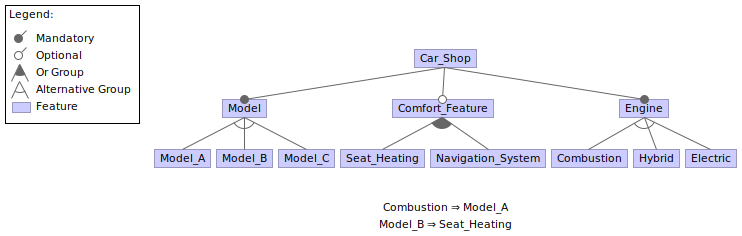
\includegraphics[scale=0.55]{gfx/Car_Shop.png}
    \caption{A feature diagram of a car dealership.}
    \label{fig:car}
\end{figure}

%What is a feature diagram and relation between features
A feature diagram is conceptually built as a tree where each node of the tree represents a feature, 
for which edge between a parent node and a child usually implies that the parent is a more general concept and the child a specialization. 
So, the further we descend in the tree, the more specialized the feature gets; with regard to its subtree.

%Feature diagram example
\autoref{fig:car} is an example for a feature diagram that depicts the structure of a car dealership. We see that the root
node \textit{car\_shop} represents the overall system. As we descend we look at the child nodes of the
\textit{Engine} feature, we can see concrete engine types, such as \textit{Combustion}, \textit{Hybrid}, and \textit{Electric}.

%Concrete and abstract feature with example
We differentiate between two types of feature nodes: \emph{abstract} and \emph{concrete} feature. 
Abstract features are used to structure the diagram, as such they not correspond to a concrete implementation.
In contrast, concrete features reflect variability inside the system, where a concrete feature is bound to an implementation artifact~\cite{Feature-Oriented-Software-Product-Lines}.

In \autoref{fig:car}, the feature \textit{Engine} is considered an abstract feature since it does not implement anything and 
is only used to give the feature diagram more structure by grouping all kinds of engines a car can possess and signaling 
the user that he must select a specific engine.
The specific engines, like \textit{Combustion} are concrete features that implement specific types of functionality.

%Mandatory and optional feature
Each feature contains a graphical notation indicating whether the feature is mandatory or optional. 
If the feature is mandatory, it is indicated with a black bubble any if it is optional, it is displayed with an empty bubble~\cite{Feature-Oriented-Software-Product-Lines-Feature-models}. 
In \autoref{fig:car}, we can see that \textit{Engine} and \textit{Model} are mandatory features, which make sense given that they are are necessary for any car 
but \textit{Comfort\_Feature} is optional and not necessary for a car to function.

%Alternative and choice groups
In addition to mandatory and optional features, there are alternative and choice groups. 
A parent can have one of the groups the alternative group is marked with an empty half circle and the choice group with a filled circle. 
When we use a choice group, one feature must be selected, but others can also be selected. Therefore, the choice group corresponds to the logical \textit{or} operator. 
In an alternative group, we can select only one feature; the configuration is invalid if more than one feature is selected~\cite{Feature-Oriented-Software-Product-Lines-Feature-models}. 
In \autoref{fig:car}, we see that \textit{Engine} has an alternative group, since each car can only contain one \textit{Engine}, 
whereas it makes sense that \textit{Comfort\_Feature} contains a choice group: one can have a navigation system and seat heating in a car without conflict.

%Constraints
A feature diagram may contain various constraints that need to be satisfied, defined as boolean algebra. In \autoref{fig:car}, we see two constraints, 
$Combustion \implies Model\_A$ and $Model\_B \implies Seat\_Heating$. The reason for such constraints could be that \textit{Model\_B} 
is a luxury model that only gets shipped with seat heating.

%Propositional formula , why useful
We use a feature model to check whether a configuration 
is valid, which is particularly useful if we want to sample or enumerate all valid configurations~\cite{Feature-Oriented-Software-Product-Lines-Feature-models}. 
\section{Performance-influence models}\label{ch:performance-influence-models}
%We explain why we introduce perf-inf models to model non-functional 
In the previous section, we introduced a way to represent variability by using feature models.
However, while doing so we ignored the non-functional properties which are as important for configurable software systems.
To model the measurable non-functional properties and to which degree each feature influences the configurable system,
we introduce \emph{performance-influence models}. 
A {\perfInfluenceModel} is a polynomial consisting of several terms, each representing either a feature or an interaction between features.
The coefficient in each term represents the degree to which these features influence the system.  
The sum of all terms represents the time the {\perfInfluenceModel} predicts given a configuration of features~\cite{Performance-influence-models-for-highly-configurable-systems}.

%Definition
Formally, let $\mathcal{O}$ be the set of all configuration options and $\mathcal{C}$ the set of all configurations, 
then let $\emph{c} \in \mathcal{C}$ be a function $\emph{c} \textit{ : } \mathcal{O} \implies \emph{\{0, 1\}}$ that assigns either $0$ or $1$ to each binary option. 
If we select a feature $o$, then $\emph{c}(\emph{o}) = 1$ holds, otherwise $\emph{c}(\emph{o}) = 0$. 
In general, a performance-influence model is a function $\Pi$ that maps configurations $\mathcal{C}$ to a prediction, 
therefore $\Pi \textit{ : } \mathcal{C} \implies \mathbb{R}$~\cite{Performance-influence-models-for-highly-configurable-systems}. 

We encode all our features as binary features and distinguish between single features $o$ denoted as $\phi_o$ and feature interactions $i ... j$ denoted as $\Phi_{i...j}$. 
Based on these definitions, we define a performance-influence model formally as~\cite{Performance-influence-models-for-highly-configurable-systems}:

\begin{gather}
    \Pi = \beta_0 + \sum_{i \in \mathcal{O}} \phi_i(c(i)) + \sum_{i...j \in \mathcal{O}} \Phi_{i...j}(c(i)...c(j))
\end{gather}

%Definition 
While $\beta_0$ denotes the base performance, which refers to the time taken by the system regardless of configuration, $\sum_{i \in \mathcal{O}} \phi_i(c(i))$ 
is the sum of each feature and $\sum_{i...j \in \mathcal{O}} \Phi_{i...j}(c(i)...c(j))$ is the sum of each feature interaction~\cite{Performance-influence-models-for-highly-configurable-systems}.

\lstset{style=myStyle}
\begin{minipage}{\linewidth}
\begin{lstlisting}[caption={Example code of a simple configurable software system that contains 4 features},language=C++,label={lst:performanceExample},escapechar=|]
void foo() {
    bool A, B, C, D; | \label{line:feature_declatation} |
    assign_feature(A, B, C, D); //Assigns the user-specified value to each feature | \label{line:featureInteraction} |
    
    fpcsc::sleep_for_secs(2); //Spending time in base feature | \label{line:feature_base} |
    if(A)                         | \label{line:feature_A_statement} |
        fpcsc::sleep_for_secs(1); | \label{line:feature_A} |
    if(B)
        fpcsc::sleep_for_secs(2); | \label{line:feature_B} |
    if(C)
        fpcsc::sleep_for_secs(1); | \label{line:feature_C} |
    if(D)
        fpcsc::sleep_for_secs(2); | \label{line:feature_D} |
    if(A && B)                    | \label{line:feature_A_B} |
        fpcsc::sleep_for_secs(2); | \label{line:feature_A_B_exec} |
    if(C && D)
        fpcsc::sleep_for_secs(0); | \label{line:feature_C_D} |
}
\end{lstlisting}
\end{minipage}

In \autoref{lst:performanceExample} we see a simple code snippet with some features that affect the performance in different ways.
In \autorefLine{line:featureInteraction}, four features \emph{A}, \emph{B}, \emph{C}, and \emph{D}, 
are declared, each of which can either be \emph{true} or \emph{false} depending on the configuration chosen.
\autorefLine{line:feature_A}, \ref{line:feature_B}, \ref{line:feature_C}, \ref{line:feature_D} will only be executed if the corresponding features are selected. 
If this is the case, the system sleeps for the specified time. 
In \autorefLine{line:feature_A_B}, we have a feature interaction where \{\emph{A}, \emph{B}\} must be selected in order for \autorefLine{line:feature_A_B_exec} to be executed, 
we would attribute the time spent in \autorefLine{line:feature_A_B_exec} to the feature interaction \{\emph{A}, \emph{B}\} and not to either feature alone.
The performance-influence model for our system would look as follows:
\begin{equation}\label{equ:performanceExamplePIMBaseline}
    \Pi = 2 + 1 \cdot c(A) + 2\cdot c(B) + 1\cdot c(C) + 2\cdot c(D) + 2 \cdot c(A)\cdot c(B) + 0\cdot c(C) \cdot c(D)
\end{equation}

For simplicity, let us assume that the execution of the code takes no time at all, and we spend no time in any feature except the time specified in the 
\textit{sleep\_for\_seconds} function.
The constant 2 here refers to $\beta_0$, the time we spend in our base feature in \autorefLine{line:feature_base}.
If we decide on the configuration \{\emph{A}, \emph{B}, \emph{C}, \emph{D}\} the model would evaluate like this:
\begin{align*}
    \Pi &= 2 + 1 \cdot c(A) + 2\cdot c(B) + 1\cdot c(C) + 2\cdot c(D) + 2 \cdot c(A)\cdot c(B) + 0\cdot c(C) \cdot c(D) \\
    \Pi &= 2 + 1 \cdot 1 + 2 \cdot 1 + 1 \cdot 1 + 2 \cdot 0 + 2 \cdot 1 \cdot 1 + 0 \cdot 1 \cdot 0 \\
    \Pi &= 2 + 1 + 2 + 1 + 2 + 2 \\
    \Pi &= 10
\end{align*}

Thus, for the configuration containing \{\emph{A}, \emph{B}, \emph{C}, \emph{D}\} our performance-influence model would predict an expected time of 10 seconds.

%************************************************
\section{Black-Box Analysis}\label{ch:Blackbox}
%************************************************
In this section, we introduce the first method we use to analyze configurable software systems, the black-box analysis. 
In \autoref{ch:bb-general-concept}, we explain a black-box and the concepts behind the black-box analysis. 
We proceed in \autoref{section:combinatorial-explosion} to explain the challenges we encounter when using a black-box analysis.
After collecting data, we use them with multiple linear regression to build a performance-influence model in \autoref{ch:linear-regression}.

\subsection{General Concepts}\label{ch:bb-general-concept}

%Introduction why now black-box
We have introduced {\perfInfluenceModel} to represent the influence of each feature and feature interaction on a system. In this section, 
we expand on this topic and introduce the \emph{black-box analysis} a method to collect data to build \perfInfluenceModel.

%What is a black-box and what is the analysis
A black-box of a configurable system is conceptually simple, we execute a given system with a configuration, and after finishing, we receive an output. 
However, the critical part is that we are unaware of how the black-box produces the output. 
Since we cannot see inside the system, we need an approach that does not require this. 
Therefore, in a black-box analysis, we solve this issue by observing the machine on which the system is executed.

\begin{figure}[h]
    \centering
    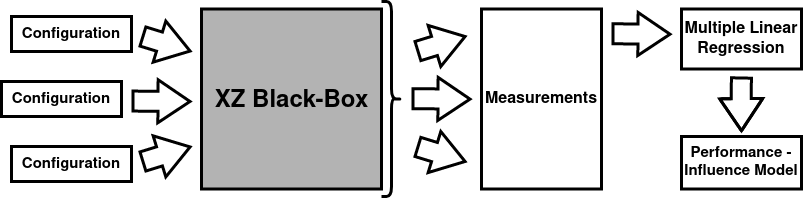
\includegraphics[scale=0.55]{gfx/BlackBox2_0.png}
    \caption{Process of using a black-box analysis to build a \perfInfluenceModel for \textit{XZ}.}
    \label{fig:BBxz}
\end{figure}

%Example of Chapter pipeline
In \autoref{fig:BBxz}, we use a black-box analysis for \textit{XZ} to build a \perfInfluenceModel.
We start by focusing on finding the features that we are interested in. 
Then we build ourselves multiple configurations that hold different interactions between these features.
Afterward, we run \textit{XZ} as a black-box on each configuration; during the execution, we analyze the system by measuring different non-functional properties.
In our case, we are interested in the performance of each feature. 
We repeat this process for each configuration during the black-box analysis and collect the measurements.
Next, we use these measurements together with multiple linear regression to build a \perfInfluenceModel.

\subsubsection{Black-Box Analysis}\label{ch:Black-Box-Analysis}

%Intro in section, combinatorial explosion
Before we start analyzing the system, we first have to select the features we are interested in, since for most configurable systems it is 
not feasible to use the whole configuration space due to its size. This issue is called \emph{combinatorial explosion} in \autoref{section:combinatorial-explosion}
we explain how we deal with this problem.

%The analysis
After deciding which features are of interest to us, we can now turn to the question 
of how we analyze the system and collect the data we need to build a \perfInfluenceModel

As shown in \autoref{fig:BBxz}, we cannot analyze how the system produces the output; 
therefore, we are limited to the non-functional properties we can observe from the outside. For this reason, 
we execute the system with each configuration and measure the property we are interested in, such as energy consumption, memory usage, 
and computational resources used.  

\subsection{Challenges}\label{section:combinatorial-explosion}
%Defining combinatorial explosion
One of the larger problems we face when using black-box analysis is the issue of combinatorial explosion, 
which refers to the effect that when features increase linearly, the number of possible configuration
increase exponentially~\cite{Combinatorial-explosion}.

%Explaining exponential groth more in detail
Suppose we have a configurable system where each feature is a binary option.
We also define that in this system, each feature is entirely independent of another
(i.e., the system has no constraints, and selecting or deselecting one feature has no effect on other features).
The number of unique configurations this system can produce is $2^n$, where $2$ refers to the type of feature options allowed,
binary in our case, and $n$ denotes the number of features. 

%Why it is a problem, Example
Here is the problem, because all these different features can interact with each other in different ways, and for very small systems
we can certainly brute-force our way by benchmarking all possible configuration, however this does not scale, and certainly not feasible for 
larger systems. For example, the Linux kernel contains 10`000 different features~\cite{Linux-Kernel}, for reference it is estimated that the universe
contains about $10^{79}$ atoms, which is still less than the number of unique configurations a system with 263 features produces, it is already impossible to use brute-force to analyze
such a system, let alone the Linux kernel.

%How wo overcome it
Hence, we cannot fully explore the entire configuration space and must select a subset representing the system with high accuracy. 
For this purpose, we take advantage of the findings of Xu et al.~\cite{TooManyKnobs}, 
where they have shown that not all features are equally important and that up to 54,1\% of features are rarely set by users. 
We use this information with our domain knowledge to extract the most important features we are interested in.


\subsection{Multiple Linear Regression} \label{ch:linear-regression}
%Section overview
After collecting all our measurements, we use them to build our {\perfInfluenceModel} of the system. 
This section explains the reasoning behind using \emph{multiple linear regression}. 
Afterward, in \autoref{ch:OLS}, we explain \emph{ordinary least squares}, an estimator to calculate the coefficient of each term inside the \perfInfluenceModel. 
While using \emph{ordinary least squares}, we have to handle the problem of \emph{multicollinear features}; we do this in \autoref{ColinearF}. 
To reduce the degree of \emph{multicollinear features} we introduce the \emph{Variance Inflation Factor} in \autoref{ch:vif}.

%Why Multiple limear regression
When building a \perfInfluenceModel from our black-box data we have the requirement that the model needs to be interpretable. While multiple 
methods to predict performance have been introduced, such as neural networks, they lack the interpretability of the model, which on contrary
\emph{multiple linear regression} provides.

To illustrate why interpretability is important lets inspect the following \perfInfluenceModel:

\begin{align*}
    \Pi_1 &= -1000 + 1001 \cdot \textit{Feature\_A} + 1002 \cdot \textit{feature\_B} - 1000 \cdot \textit{Feature\_A} \cdot \textit{feature\_B} \\
    \Pi_2 &= 0 + 1 \cdot \textit{Feature\_A} + 2 \cdot \textit{feature\_B} + 0 \cdot \textit{Feature\_A} \cdot \textit{feature\_B}
\end{align*}

%Example why we need interpretability
Under the condition that either \textit{Feature\_A} or \textit{Feature\_B} needs to be selected, 
$\Pi_1$ and $\Pi_2$ predict for any configuration the same amount of time, however, 
if we take a close look at how $\Pi_1$ assigns the influence of each feature, we can see that this is not interpretable. 
Here $\Pi_1$ assigns to the \textit{Base} feature an influence of -1000 thousand, 
which does not make sense since the time spent in the \textit{Base} feature can not be negative. 
This also leads to $\Pi_1$ assigning unrealistic amounts of time to features or feature interactions. 

We use the following formula for linear regression for matrices ~\cite{Linear-Regression-Performance}:

\begin{align}\label{formula:linReg}
    Y &= \beta_0 + \beta_1 x_1 + \beta_2 x_2 ... \beta_n x_n + \epsilon   \\
    Y &= X \beta + \epsilon \nonumber\\ \nonumber \\ \nonumber
    Y &= \textit{Dependent variable}\\ \nonumber
    X &= \textit{Independent variable}\\ \nonumber
    \beta &= \textit{Regression coefficient}\\ \nonumber
    \epsilon &= \textit{Error} \nonumber
\end{align}

%For what linear reg is used
The model is used to estimate the relationships between the independent variables and the dependent variable.
In our case, $Y$ is a vector with \textit{n}  elements containing the output of our black-box model,
i.e., the measurements for each configuration in our set of configurations $\mathcal{C}$. 

%Exlaining collums of matrix and how they map to our config
Our independent variable $X$ is an $n \times m$ matrix, where $n$ is the number of configurations used, 
and $m$ is the number of features and feature interactions across all configurations. 
To accommodate feature interactions in this linear model, we add a term for each interaction we want to include. 
For example, if we consider the interaction between features $x_i$ and $x_j$ we add the term $\beta_k x_i x_j$. 

%Explaining coecfficient map to feature
We are interested in the values of the coefficients $\beta$, since they quantify the influence of each feature or feature interaction on the whole system. 
In addition, $\beta_0$ denotes the intercept, representing the influence of the base code, 
meaning the part of the code executed regardless of the chosen configuration.

%Splitting of feature interactions
The value of each feature in the matrix is $1$ if the feature is selected or $0$ if it is not selected.  If we have numerical features with $l$ different options, 
we split these features into $l$ binary features and encode them as an alternative group in our feature model.

%Error
All our measurements have a possible error represented by $\epsilon$~\cite{Linear-Regression}.

\subsubsection{Ordinary Least Squares}\label{ch:OLS}
%Why we need ols
Now that we have seen the general formula of multiple linear regression and know what the different components stand for, we still need to figure out 
how to calculate the regression coefficient $\beta$, the values that tell us the influence of each feature. 

%Why OLS works in detail
For this purpose, we use the ordinary least squares estimator, which is optimal for the class of linear unbiased estimators, 
but is unreliable when the independent variables $X$ contains a high degree of multicollinearity, we explain this in detail in \autoref{ColinearF}.
The principal of ordinary least squares is to minimize the sum of the squared residuals, where the residual is the difference between
the predicted value of the estimator and the actual value.~\cite{Linear-Regression}


\begin{figure}[H]
    \centering
    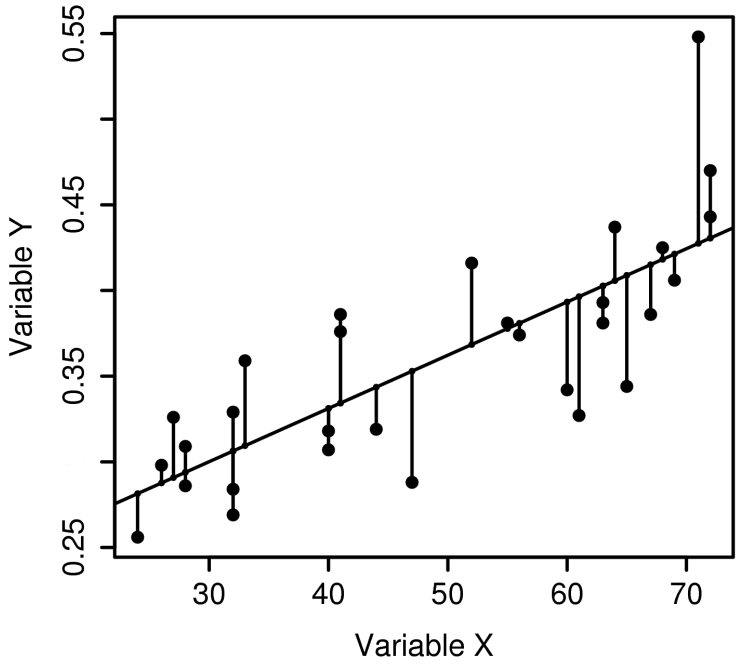
\includegraphics[scale=0.3]{gfx/OLS.png}
    \caption[Ordinary Least Squares regression model residuals]
    {Ordinary Least Squares regression model residuals
    \footnotemark}
    \label{fig:OLS}
\end{figure}
\footnotetext{Visited at 06.03.2023, \url{https://datajobs.com/data-science-repo/OLS-Regression-[GD-Hutcheson].pdf}}

%example illustration
We see an illustration of an ordinary least squares estimator for a linear regression model in \autoref{fig:OLS}, where we have only one variable 
X and the corresponding measurements Y, allowing us to compute the single regressor for this linear regression model.

To compute the regression coefficients using ordinary least squares, the following formula is used~\cite{Linear-Regression}:

\begin{align}
    \hat{\beta} &=  (\textit{X}^{\top } \textit{X} )^{-1}\textit{X}^{\top} Y \\ \nonumber \\\nonumber
    \hat{\beta} &= \textit{Ordinary Least Squares estimator}\\\nonumber
    \top &= \textit{Matrix Transposed}\nonumber
\end{align}\label{equ:ols}

Now $\hat{\beta}$ contains the regression coefficient we are interested in.

As an example, we can refer to our code from \autoref{lst:performanceExample}
and sample some configurations to build a multiple linear regression model using ordinary least squares.

\begin{table}[H]
    \centering
    \begin{tabular}{rrrrrrrr}
    \hline
    Base & A & B & C & A $\land$ B & A $\land$ C &  & $\bm{\Pi(*)}$ \\ \hline
    1    & 0 & 0 & 0 & 0           & 0           &  &  $\mathbf{1}$   \\
    1    & 1 & 0 & 0 & 0           & 0           &  &  $\mathbf{2}$   \\
    1    & 0 & 1 & 0 & 0           & 0           &  &   $\mathbf{3}$  \\  
    1    & 0 & 0 & 1 & 0           & 0           &  &   $\mathbf{2}$  \\  
    1    & 1 & 1 & 0 & 1           & 0           &  &   $\mathbf{6}$   \\
    1    & 1 & 0 & 1 & 0           & 1           &  &   $\mathbf{3}$  \\  
    1    & 0 & 1 & 1 & 0           & 0           &  &   $\mathbf{4}$  \\  
    1    & 1 & 1 & 1 & 1           & 1           &  &   $\mathbf{7}$  \\ \hline

    \end{tabular}  
    \caption{Configuration samples of \autoref{lst:performanceExample}}
\end{table}

Using the configuration samples from \autoref{tab:alternative} we can now determine $\textit{X}$ and $\textit{Y}$:

\begin{displaymath}
    \textit{X} = 
    \begin{bmatrix} 
        1 & 0 & 0 & 0 & 0 & 0 \\
        1 & 1 & 0 & 0 & 0 & 0 \\
        1 & 0 & 1 & 0 & 0 & 0 \\
        1 & 0 & 0 & 1 & 0 & 0 \\
        1 & 1 & 1 & 0 & 1 & 0 \\
        1 & 1 & 0 & 1 & 0 & 1 \\
        1 & 0 & 1 & 1 & 0 & 0 \\
        1 & 1 & 1 & 1 & 1 & 1 
      \end{bmatrix}
      ,
      \textit{Y} =
      \begin{bmatrix}
        1 \\
        2 \\
        3 \\
        2 \\
        6 \\
        3 \\
        4 \\
        7 
      \end{bmatrix}
\end{displaymath}


Using the ordinary least squares \hyperref[equ:ols]{Equation \ref*{equ:ols}}  we obtain the following results:

\begin{equation}
    \hat{\beta} = 1 + 
    \begin{bmatrix}
        0,00 \\
        1,00 \\
        2,00 \\
        1,00 \\
        2,00 \\
        0,00
    \end{bmatrix}
\end{equation}

All values have been rounded to 2 decimal places. 
We can see that all values have been assigned correctly.

Now we can use the values to create the \perfInfluenceModel:

\begin{equation}\label{equ:performanceExamplePIMBlackBox}
    \Pi = 1 + 1 \cdot c(A) + 2 \cdot c(B) + 1 \cdot c(C) + 2 \cdot c(A) \cdot B + 0 \cdot c(A) \cdot c(C)
\end{equation}

\subsubsection{Multicollinear Features}\label{ColinearF}
%Connection/Explantion why multicolinearty is bad
We already mentioned that ordinary least squares is optimal as long as our configurations do not contain multicollinearity. The reason for that
is in presence of multicollinearity the variance of the estimator inflates, which in result hurts the interpretability of the model.
We call features multicollinear when there exist a near linear dependency between these features, meaning we can nearly represent one feature as a combination
of different features and the feature does only provide a small amount of new information to the system~\cite{Linear-Regression}. If a feature does not provide
any new information to the system, then we speak of perfect multicollinearity.

As an example take a look at a {\perfInfluenceModel} for some the monthly expenses of a student:
\begin{equation*}
    monthly\_expenses = \textit{food} + \textit{take\_out}
\end{equation*}

%Explanation and example for perfect multicolinearity
Now this shows multicollinearity between the features \textit{food} and \textit{take\_out}, since \textit{take\_out} is already present in the cost of \textit{food},
furthermore it is a case of perfect multicollinearity, since the feature does not provide any new information.

One way multicollinearity is introduced into a system is by using alternative groups, since the selection of a feature in the
alternative group can be expressed by the combination of all other feature.~\cite{Multicollinearity}

\begin{table}[h]
    \centering
    \begin{tabular}{llllll}
    \hline
    Base & A & B & C &  & $\bm{\Pi(*)}$ \\ \hline
    1 & 1 & 0 & 0 &  & $\mathbf{5}$  \\
    1 & 0 & 1 & 0 &  & $\mathbf{10}$  \\  
    1 & 0 & 0 & 1 &  & $\mathbf{15}$  \\\hline
    \end{tabular}  
    \caption{Configuration example illustrating multicollinearity in an alternative group.
    Where $\bm{\Pi(*)}$ is the sum of all selected features inside the row}\label{tab:alternative}
\end{table}

%Example alternative group
Now consider the example of \autoref{tab:alternative}, where we see a configuration example that contains multicollinear features due to an alternative group.
The example contains a mandatory \textit{Base} feature and 3 features in an alternative \textit{A}, \textit{B}, and \textit{C}.
Now we can always model the present of a feature in an alternative group due to the absence of other feature, here for feature \textit{C} to be selected, 
\textit{B} and \textit{A} needs to be deselected.

\begin{align*}
    \Pi_0(c) &= 0 + 5 \cdot c(A) + 10\cdot c(B) + 20\cdot c(C) \\
    \Pi_1(c) &= 5 + 10 \cdot c(A) + 5\cdot c(B) + 20\cdot c(C) \\
    \Pi_2(c) &= 8 + 20 \cdot c(A) + 10\cdot c(B) + 7\cdot c(C) \\
\end{align*}

This leads to multiple performance-influcence model that are accurate with respect to the individual measurement, 
but make completely different statements when compared.

\begin{table}[h]
    \centering
    \begin{tabular}{lllllll}
    \hline
    $\Pi$ & Base & A & B & C   & &  $\bm{\Pi(\{Base\})}$   \\ \hline
    $\Pi_0$ & 0 & 5  & 10 & 20 & &  $\mathbf{0}$         \\
    $\Pi_1$ & 5 & 10 & 5  & 20 & &  $\mathbf{5}$         \\  
    $\Pi_2$ & 8 & 20 & 10 & 7  & &  $\mathbf{8}$        \\\hline
    \end{tabular}
    \caption{Performance predictions of \autoref{tab:alternative}}\label{tab:Performance-predictions}
\end{table}

%Explain multicollinearity 
Another way multicollinearity is introduced into the system is to have features that are mandatory or connected by a condition. 
If we have features that are mandatory, we cannot distinguish these features with our black-box analysis because they are always selected
together, and we cannot determine the extent to which each feature influences the system.~\cite{Multicollinearity}

%Multicolinearity with mandatory feature explaining examples before
In \autoref{tab:Performance-predictions}, we can see the predictions each of the 3 \perfInfluenceModel make for the configurations $\{Base\}$. 
Now $\Pi_0$, $\Pi_1$, and $\Pi_2$, assign completely different values to the \textit{Base} feature, which makes it impossible for us, the user,
to identify the correct value. The reason is that both \textit{Base} and a feature of the alternative group are mandatory; 
therefore, we cannot measure one without the presence of the other. 
Hence, the values of \textit{Base} or the alternative group feature can be set in any ratio as long as the sum of the two values equals the measured time.

When we decide on which features to use in our configuration set, we use our domain knowledge of the system to reduce the amount multicollinear
features to a minimum.

%\begin{algorithm}[h]
%    \caption{Equivalence \label{alg:Colinear}}
%    \begin{algorithmic}[1]
%
%    \If{$(c \textit{ and }  \lnot d) or (\lnot c \textit{ and } d)$} 
%        \State $c,d \gets False$
%    \EndIf
%
%    \end{algorithmic}
%    \end{algorithm}
%
%By extending the example code from \hyperref[alg:performanceExample]{Algorithm \ref*{alg:performanceExample}} with an additional condition where $C \equiv D$ holds, 
%so that either C or D can be selected without the other, we insert the code snippet \hyperref[alg:Colinear]{Algorithm \ref*{alg:Colinear}} 
%after \hyperref[alg:code_insertion]{Algorithm \ref*{alg:code_insertion}}.

%Now, if we select a configuration c that contains the features \{\{A\}, \{B\}, \{C\}\} we get multiple {\perfInfluenceModel}s:

%\begin{align*}
%    \Pi_1(c) &= 1 + 1\cdot c(C) + 1 \cdot c(D) + 1\cdot c(C) \cdot c(D) \\
%    \Pi_2(c) &= 1 + 0\cdot c(C) + 0 \cdot c(D) + 3\cdot c(C) \cdot c(D) \\
%    \Pi_3(c) &= 1 + 1\cdot c(C) + 2 \cdot c(D) + 0\cdot c(C) \cdot c(D) \\
%\end{align*}

%In $\Pi_1(c)$ and $\Pi_2(c)$, all features are assigned different values from what we would expect when looking at Algorithm \ref{alg:performanceExample},
%while the \perfInfluenceModel of $\Pi_C(c)$ assigns the expected values.

\subsubsection{Variance Inflation Factor}\label{ch:vif}
In reality, multicollinearity is often unavoidable in configurable systems, when we want to model the influence of a feature interaction between features
\textit{A} and \textit{B} we introduce a term $A \cdot B$, this feature interaction is only selected when feature \textit{A} and \textit{B} are selected. 
Due to that reason we can not remove terms that introduce multicollinearity, however we can remove perfect multicollinear since they do not provide our 
system with new information.

To check for perfect multicollinearity we use the variance inflation factor (VIF), where a VIF factor of $\inf$ indicates
that there is perfect multicollinearity between features of feature interactions~\cite{Multicollinearity}.

We compute the VIF using the following equation:

\begin{align}
    VIF_{j} &= \frac{1}{1 - R^{2}_{j}}  \\ \nonumber\\
    R^{2}_{j} &= 1 - \frac{\sum\limits_{\forall c \in \mathcal{T}} (c(o_j) - \overline{c}(o_j))^2} {\sum\limits_{\forall c \in \mathcal{T}}(c(o_j) - f_j(c \setminus o_j))^2}
\end{align}

Where $\mathcal{T}$ is the trainings set containing \textit{j} features $o_j$. The VIF$_{j}$ can be calculated for each feature by using the coefficient
of determination $R^2$. To do this, we need to calculate $R^{2}_j$ for each feature $o_j$, fitting a linear regression function $f_j$ to predict whether $o_j$
is selected in the configuration $c \setminus o_j$, using all other features as predictors and the overall mean $\overline{c}(o_j)$~\cite{Multicollinearity}.

\subsubsection{Deciding which terms by using VIF}
%Explain we cant just remove all mulitcollinear term, but only those introducing perfect algorithm
Multicollinearity is present in nearly every configurable system. 
Therefore, we cannot simply remove every term that introduces multicollinearity into the {\perfInfluenceModel}. 
Therefore, we need a strategy to determine the terms we must remove. For this, we use the VIF to determine the terms that add no new information, 
meaning the features that introduce perfect multicollinearity. To accomplish this, we use the following algorithm:

\begin{algorithm}
    \caption{Iterative VIF to check for perfect multicollinearity}\label{alg:vif_iterative}
    \begin{algorithmic}[1]
    \State $\textbf{Input: } \textit{Model\_to\_check}$, list containing all the terms we want to check 
    \State $\textbf{Output: } \textit{Current\_model}$, list containing no terms that introduce perfect multicollinearity
    \State $\textit{Current\_model} \gets \textbf{[\;]}$ \textbackslash\textbackslash Initialize empty list
    \State $\textit{Current\_model.add(Model\_to\_check.pop())} $ \label{alg:vif_add_item}
    \For{$\textit{Term}\;\textbf{in}\;\textit{Model\_to\_check}$} 
        \State $\textit{Current\_model.add(Term)}$
        \If{$\infty\;\textbf{in}\;\textit{VIF(Current\_model)}$}\label{alg:vif_check} \\    
            \qquad$\textit{Current\_model.remove(Terms)}$ 
        \EndIf
    \EndFor
    \State\Return $\textit{Current\_model}$

    \end{algorithmic}
\end{algorithm}

%Explaining Algortihm
In \refAlgorithm{alg:vif_iterative}, we introduce an algorithm that removes all terms that add multicollinearity to our {\perfInfluenceModel}. 
The algorithm takes as an input $\textit{Model\_to\_check}$ a model with all the terms we want to check for multicollinearity. 
Afterward, for each $\textit{Term}$ in $\textit{Model\_to\_check}$, 
we add $\textit{Term}$ to our $\textit{Current\_model}$ and check in \autorefLine{alg:vif_check} if the term introduced multicollinearity, 
which happens if one VIF value is $\inf$, if this happens we remove $\textit{Term}$ from our $\textit{Current\_model}$. 
In the end, we return $\textit{Current\_model}$, containing all terms that do not introduce multicollinearity.

\mycomment{
    Ich würde es alles ein wenig anders strukturieren. Das sollte ohne großen inhaltlichen Mehraufwand recht simpel sein:
1. Introduction
1.1 Context/Motivation
1.2 Goals
1.3 Contributions
2. Background
2.1 Configurable Systems
2.1.1 General Concepts
2.1.2 Features and Configs
2.1.3 Functional/Non-Function Properties
2.2 Modelling Configurable Systems
2.2.1 Feature Models
2.2.2 Feature Diagrams
-> Ggf. auch keine Einteilung in explizite Unterpunkte für 2.2
2.3 Analyzing Configurable Systems
  -> Das ist dein aktuelles 2.5, da ggf. am Ende noch einen kurzen Absatz, welche Analysemöglichkeiten es gibt (BB/WB) aber detaillierte Beschreibung erfolgt in den Unterkapiteln dazu
2.4 Black-Box-Analysis
2.4.1 General Concepts
2.4.2 Challenges (Aktuell 2.6.1.1)
2.4.3 Multiple Linear Regression (Aktuell 2.6.2)
2.5 White-Box Analysis
2.5.1 General Concepts 
  -> Sollte im Endeffekt, beinhalten was du vor 2.7.1 aktuell hast + 2.7.1 + kurzer Anriss, was Feature Taints sind
2.5.2 VaRA
  -> Das was du auch aktuell zu VaRA hast. Die Unterteilung in Unterkapitel ist hilfreich, aber mMn auch nicht zwangsweise notwendig
}
%1. Intro White-box, overview of analysis
%2. Explaining some analyzing strats that are out there
%3. VaRA, explain what vara does roughly (Regions)
%4. Vara TS Experiment explain
%5  TEF Report and how we evaluate them
%6. Using data to build multiple perf-influcence models


%************************************************
\section{White-box Model}\label{ch:Whitebox}
%************************************************

While a black-box analysis is very useful for systems where we do not have access to the source code, when we do have that access
it would be a waste not to work with this additional information. This enables use to use a white-box analysis 
that takes advantage of these new information and uses them to derive a \perfInfluenceModel differently then the black-box approach.


\begin{figure}[h]
    \centering
    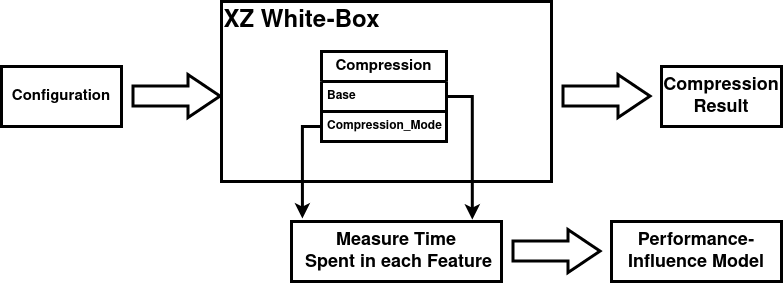
\includegraphics[scale=0.6]{gfx/whitebox_2.png}
    \caption{A white-box analysis of XZ}
    \label{fig:WBxz}
\end{figure}

We now analyze the example system from \autoref{fig:xz} using a white-box analysis. In \autoref{fig:WBxz} we can now see the inner workings of 
XZ when we are compressing a file. During the compression we can measure the time XZ spent in its various features, in our example we measure 
the time spent in $Base$ and $Compression_Model$, after system finished the process of compression we collected all measurements which we 
then use to build a \perfInfluenceModel for that configuration.

In this section we explain current state-of-the-art strategies and which principles they deploy to collect the measurements of each feature 
\ref{analyzing-strats}. We then proceed to explain which analyzing tool we use, a variability aware region analyzer and the underlying principles
behind it \ref{VaRA}. Afterwards we will aggregate the data that we collected to build a \perfInfluenceModel. % Ref TEF/Perf



%\subsection{Disadvantages of White-Box}
%When using white-box model we clearly see how a feature interacts with another feature, due to that we do not need to sample our configuration space like
%we do in the black-box, meaning we do not face the problem of combinatorial explosion. 
%Neither do we have to handle multicollinearity features differently, since we can see in what extend they influence each other. 
%The example from \ref{ColinearF} would be no problem for the white-box model since we are aware that $c$ and $d$ do not interact with one another and can
%therefore assign them the precise amount of time they spend in their code region respectively, whereas the black-box model needs to infer this information.

%With the surplus of information, the white-box model faces different challenges. 
%First and foremost, to analyze larger systems we need a robust strategy and in depth code comprehension.

\subsection{Analyzing Strategies}\label{analyzing-strats}
Analyzing programs is a highly complex topic in itself, it is not a trivial task to use a program to run an analysis over a different system.
In our case, we first need to find out which parts of the code corresponds to which feature.

To solve this problem multiple solutions have been proposed, Weber et. al. \cite{White-box-Profiling} uses a profiling approach, to generate 
performance-influence models that depict configurability on a method level, to achieve this they first used a JProflier a coarse-grained profiler
to learn a performance influence model for every method that have been learned successfully. 
To identify the methods that are hard to learn they use a filtering techniques, afterwards using KIEKER a fine-grained profiler to learn these methods.

Velez et. al. introduced us to ConfigCrusher \cite{ConfigCrusher} a white-box analysis, that uses a static data-flow analysis to see how features influence 
variables and the control-flow of the system. In addition, ConfigCrusher uses three insights about configurable systems, from previous works, namely
irrelevance, orthogonality and low interaction degree. Irrelevance, is used to identify the features that are relevant for the data-flow of the system, and by
doing so reducing the amount of configurations necessary to analyze the system. Orthogonality, is used to identify features that do not influence each other, and
thus can be measured together. Low interaction degree, is used to identify the relevant feature interaction, since only few features interact with another, 
ConfigCrusher focuses on those configurations with interacting features to reduce the amount of configuration that need to be sampled. 
Out of these insights two techniques are developed, namely compression and composition.
Compression is used to reduce the number of configurations necessary to analyze the system,
by simultaneously analyzing regions that are independent of another, therefore they can use a single configuration to 
analyze different features. 
They take advantage of the fact that \perfInfluenceModel can be build compositionally, by generating a performance-influcence model for each region separately
and afterwards compose all the local \perfInfluenceModel into a model for the whole system.

Siegmund et. al. introduced us to Comprex \cite{Comprex} which uses a dynamic taint analysis to identify how
and to what degree features influence the control-flow of the given system. 

Both Comprex and ConfigCrusher use the techniques of compression and composition, the major difference between both analysis methods is Comprex uses a dyanmic taint
analysis, whereas ConfigCrusher uses a static data-flow analysis, both are used to depict configurability on a feature level, where Weber et. al. depicts
configurability on a method level instead. 

After figuring out which parts of the code corresponds to what feature we still need to instrumentalize the code 

\subsection{VaRA}\label{VaRA}
To analyze the system we are interested in we use VaRA a variability aware region analyzer, a framework build on LLVM to analyze software
and the VaRA Tool Suite\footnote{Visited at 14.03.2022 \url{https://vara.readthedocs.io}}, developed at Saarland University. 

VaRA is able to 
detect which code regions are influenced by which feature using a data-flow analysis. Afterwards the code gets instrumentalized to measure the time
spent in each region. \cite{VaRA-Flo}

\subsubsection{VaRA Tool Suite}
We use VaRA in combination with the VaRA Tool-Suite which enables us to use VaRA by specifying an experiment to analyze a specific project. 

An experiment inside the VaRA Tool-Suite is a concept which specify how we want to analyze a software project, this allows us to make the analysis
easy to reproduce and repeat. The project specifies the system we want to analyze, here we  define how we build the system or which version we 
of the system we are interested in. 

For our example of \autoref{fig:WBxz}, the project would be XZ and would specify which version of xz we want to analyze and how the binary is build.
The experiment defines which configuration we want to analyze in addition to how we would like to analyze it, in our case we want to analyze 
XZ using VaRA, we also specify in what format we would like to have our measurements stored, such as the Trace Event Format in \ref{trace-event}.

\subsection{Trace Event Format}\label{trace-event}
When we analyze a system it is very rare that we only enter the region of a feature once and afterwards stop interacting with that feature. 